\documentclass{beamer}
\usepackage{graphicx}
\usetheme{metropolis}


\title[WebAssembly]{WebAssembly}
\author{Jakob Waibel}
\institute[Jakob Waibel]{MI7 Druck und Medien}
\date

\begin{document}

\begin{frame}
    \titlepage
\end{frame}

\begin{frame}
    \frametitle{Agenda}
    \tableofcontents
\end{frame}

\section{Einführung}

\begin{frame}{Motivation}
    \begin{figure}
        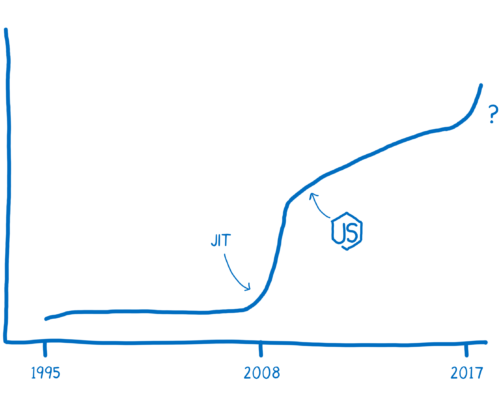
\includegraphics[width=0.7\textwidth,height=0.7\textheight]{./images/perf_history.png}
        \caption{\href{https://hacks.mozilla.org/2017/02/a-cartoon-intro-to-webassembly/}{Performance-Entwicklung im Web-Kontext}}
    \end{figure}
\end{frame}

\begin{frame}{Definition}
    \begin{figure}
        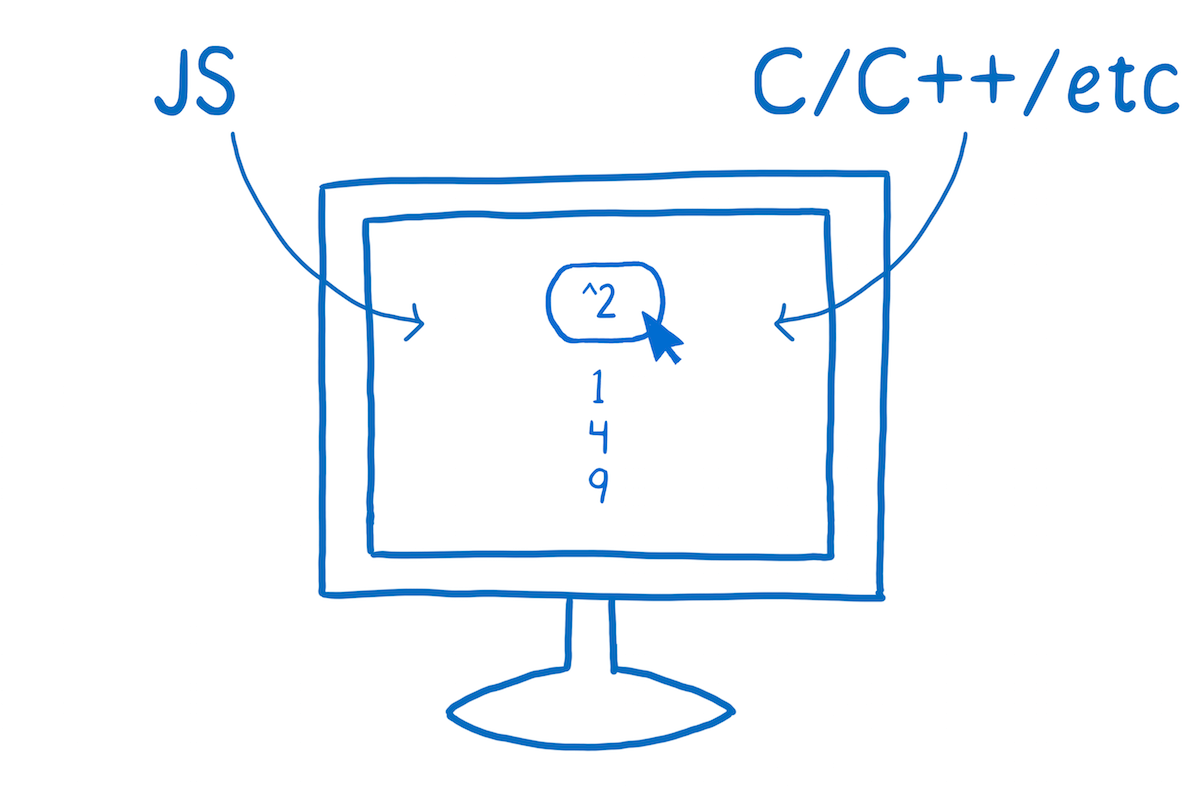
\includegraphics[scale=0.2]{./images/definition.png}
        \caption{\href{https://www.smashingmagazine.com/2017/05/abridged-cartoon-introduction-webassembly/}{Introduction to WebAssembly}}
    \end{figure}
\end{frame}

\begin{frame}{Definition}
    \begin{figure}
        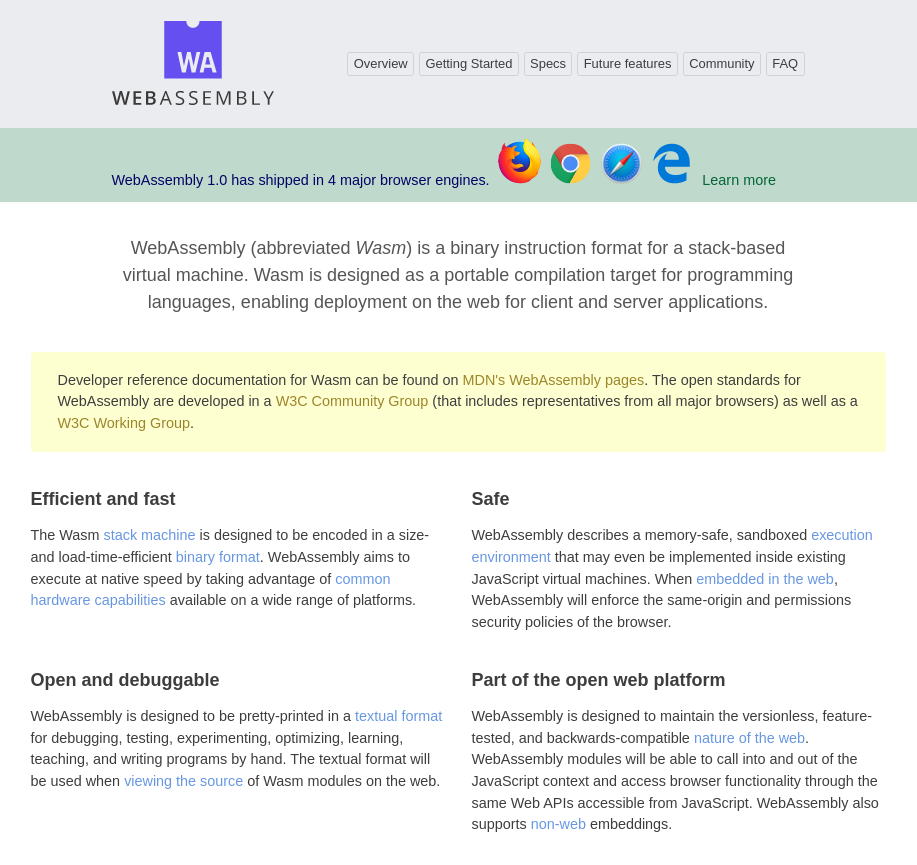
\includegraphics[scale=0.2]{./images/webassembly_org.png}
        \caption{\href{https://webassembly.org/}{webassembly.org}}
    \end{figure}
\end{frame}

\begin{frame}{Definition}
    \begin{quotation}
        "\textbf{WebAssembly} (abbreviated Wasm) is a \textbf{binary instruction format} for a \textbf{stack-based virtual machine}. Wasm is designed as a \textbf{portable compilation target} for programming languages, \textbf{enabling deployment on the web} for client and server applications."
    \end{quotation}
\end{frame}

\begin{frame}{Binary Instruction Format}
    \begin{itemize}
        \item Machine instruction format consisting of \textbf{1s and 0s} that can be directly decoded and \textbf{executed by the CPU}
        \item \textbf{Targeting different instruction set architectures} (ISA) like x86, ARM or RISC-V
        \item WASM uses \textbf{virtual instructions} for a \textbf{conceptual machine}, not a physical one
        \item Think of WASM instruction set as "intersection" of multiple ISAs that can't be mapped directly to one ISA
    \end{itemize}
\end{frame}

\begin{frame}{Stack-Based Virtual Machine}
\end{frame}

\begin{frame}{Portable Compilation Target}
\end{frame}

\begin{frame}{Deployment on the Web Platform}
\end{frame}

\end{document}